% ==============================================================================
% SECAO 5 — PROJETO DOS CONTROLADORES E ANALISE FREQUENCIAL
% ==============================================================================
\section{PROJETO DOS CONTROLADORES P, PI, PD E PID E ANÁLISE FREQUENCIAL}\label{sec:projeto_comp}

Identificadas as limitações do ganho proporcional na Seção~\ref{sec:controle_p}, esta seção formaliza os requisitos de desempenho, projeta os controladores P, PI, PD e PID e examina suas propriedades no plano complexo e no domínio da frequência.

\subsection{Síntese dos Requisitos de Desempenho}\label{sec:requisitos}
Os controladores P, PI, PD e PID são projetados visando reduzir a fila de $600$ para $300\text{ eventos}$ ($x_r = 300\text{ eventos}$), atendendo a seis especificações operacionais: tempo de subida $t_r(10\%\text{--}90\%) \le 5\text{ s}$; tempo de acomodação $t_s(2\%) \le 12\text{ s}$; sobressinal máximo $M_p \le 10\%$; erro em regime permanente $e_{ss} \le 10\text{ eventos}$ (inclusive após a perturbação $\Delta\lambda = +100\text{ eventos/s}$); margem de fase ($\mathrm{PM}$, do inglês \textit{phase margin}) $\mathrm{PM} \ge 45^\circ$; e capacidade efetiva restrita ao intervalo $\mu(t) \in [600,\,1400]\text{ eventos/s}$.

\subsection{Funções de Transferência dos Controladores e Malhas Fechadas}\label{sec:fts_comp}
Considerando a planta $G(s) = \frac{1}{s(2s+1)}$ com realimentação unitária negativa, cada controlador $C(s)$ define a função de transferência de referência $T(s) = C(s)G(s)/[1+C(s)G(s)]$ e a função de transferência da perturbação $T_d(s) = X(s)/\Delta\Lambda(s) = -(2s+1)/[s(2s+1)+C(s)]$ (FRANKLIN; POWELL; EMAMI-NAEINI, 2013). Com o controlador proporcional, $C_{\text{P}}(s) = K_p$, o polinômio característico permanece de segunda ordem:
\begin{equation}
    T_{\text{P}}(s) = \frac{K_p}{2s^2 + s + K_p}, \qquad T_{d,\text{P}}(s) = -\frac{2s+1}{2s^2 + s + K_p}.
\end{equation}
A ação integral, $C_{\text{PI}}(s) = K_p + K_i/s = (K_p s + K_i)/s$, eleva a ordem do sistema para três, acrescenta um zero em $-K_i/K_p$ e introduz em $T_d(s)$ um zero na origem, que é o responsável pela rejeição da perturbação em degrau:
\begin{equation}
    T_{\text{PI}}(s) = \frac{K_p s + K_i}{2s^3 + s^2 + K_p s + K_i}, \qquad T_{d,\text{PI}}(s) = -\frac{s(2s+1)}{2s^3 + s^2 + K_p s + K_i}.
\end{equation}
O controlador PD é tratado na forma ideal $C_{\text{PD}}(s) = K_p + K_d s$ na sintonia analítica e na forma realizável $C_{\text{PD,f}}(s) = K_p + K_d s/(\tau_f s+1)$, com $\tau_f = 0{,}05\text{ s}$, nas simulações. Na forma ideal, a ação derivativa altera apenas o coeficiente de primeira ordem do polinômio característico:
\begin{equation}
    T_{\text{PD}}(s) = \frac{K_d s + K_p}{2s^2 + (1 + K_d)s + K_p}, \qquad T_{d,\text{PD}}(s) = -\frac{2s+1}{2s^2 + (1 + K_d)s + K_p}.
\end{equation}
O controlador PID reúne as três ações, $C_{\text{PID}}(s) = (K_d s^2 + K_p s + K_i)/s$, e nas simulações adota a mesma forma filtrada $C_{\text{PID,f}}(s) = K_p + K_i/s + K_d s/(\tau_f s+1)$. Na forma ideal,
\begin{equation}
    T_{\text{PID}}(s) = \frac{K_d s^2 + K_p s + K_i}{2s^3 + (1 + K_d)s^2 + K_p s + K_i}, \quad T_{d,\text{PID}}(s) = -\frac{s(2s+1)}{2s^3 + (1 + K_d)s^2 + K_p s + K_i},
\end{equation}
cada coeficiente do polinômio característico passa a depender de um ganho diferente. É essa propriedade que permite a alocação arbitrária dos três polos na Seção~\ref{sec:sintonia}.

\subsection{Sintonia Analítica e Justificativa Matemática dos Ganhos}\label{sec:sintonia}

\subsubsection{Controlador P ($K_p = 0{,}369$)}
Seleciona-se o ganho de referência ligeiramente acima do limiar de $10\%$ de sobressinal ($M_p = 10{,}55\%$), em que $\zeta \approx 0{,}582$ pela Equação~\eqref{eq:wn_zeta_p}, resultando nos polos $s_{1,2} = -0{,}25 \pm j0{,}349\text{ s}^{-1}$.

\subsubsection[Controlador PI (caso estável e caso instável)]{Controlador PI ($K_p = 0{,}350,\; K_i = 0{,}030$ e caso instável $K_p = 0{,}500,\; K_i = 0{,}300$)}
Pelo critério de Routh-Hurwitz aplicado à equação característica $2s^3 + s^2 + K_p s + K_i = 0$ (OGATA, 2010):
\[
\begin{array}{c|cc}
    s^3 & 2 & K_p \\
    s^2 & 1 & K_i \\
    s^1 & K_p - 2K_i & 0 \\
    s^0 & K_i & 0
\end{array}
\]
a estabilidade exige $K_p > 0$, $K_i > 0$ e $K_i < K_p / 2$. Para limitar a degradação de fase em $\omega_{cp}$ e buscar $\mathrm{PM}$ próxima de $45^\circ$, posiciona-se o zero do PI em $z_{\text{PI}} = -K_i/K_p \approx -0{,}086\text{ s}^{-1}$ (bem abaixo da frequência de cruzamento), adotando $K_p = 0{,}350$ e $K_i = 0{,}030 < 0{,}175$. Adicionalmente, para evidenciar na Seção~\ref{sec:limitacoes_comp} a transição ao semiplano direito prevista por Routh-Hurwitz, analisa-se a configuração instável $K_p = 0{,}500,\; K_i = 0{,}300 > 0{,}250$.

\subsubsection[Controlador PD ($K_p = 1{,}280,\; K_d = 1{,}560$)]{Controlador PD ($K_p = 1{,}280,\; K_d = 1{,}560$, $\tau_f = 0{,}05\text{ s}$)}
Igualando a equação característica normalizada $s^2 + \frac{1+K_d}{2}s + \frac{K_p}{2} = 0$ ao polinômio desejado de segunda ordem $s^2 + 2\zeta\omega_n s + \omega_n^2 = 0$, obtêm-se as equações de alocação de polos (NISE, 2017):
\begin{equation}
    K_p = 2\omega_n^2, \qquad K_d = 4\zeta\omega_n - 1.
\end{equation}
Escolhendo $\omega_n = 0{,}80\text{ rad/s}$ e $\zeta = 0{,}80$ (de modo a manter tempo de subida rápido $t_r \approx 1{,}8/\omega_n \approx 2{,}2\text{ s}$ e zero suficientemente afastado dos polos dominantes, $z_{\text{PD}} = -K_p/K_d = -0{,}821\text{ s}^{-1}$, para limitar o sobressinal adicional), obtém-se $K_p = 2(0{,}80)^2 = 1{,}280$ e $K_d = 4(0{,}80)(0{,}80) - 1 = 1{,}560$.

\subsubsection[Controlador PID nominal e sintonia ajustada ($\alpha = 0{,}40\text{ s}^{-1}$)]{Controlador PID nominal ($K_p = 2{,}160,\; K_i = 0{,}243,\; K_d = 2{,}900$, $\tau_f = 0{,}05\text{ s}$) e sintonia ajustada sob saturação ($\alpha = 0{,}40\text{ s}^{-1}$)}
Utiliza-se a alocação exata de polos de terceira ordem impondo o polinômio característico desejado com um par criticamente amortecido ($\omega_n = 0{,}90\text{ rad/s}$, $\zeta = 1{,}0$) e um polo real associado à ação integral ($\alpha$) (FRANKLIN; POWELL; EMAMI-NAEINI, 2013):
\begin{equation}
    (s + \alpha)(s^2 + 2\zeta\omega_n s + \omega_n^2) = s^3 + (\alpha + 2\zeta\omega_n)s^2 + (\omega_n^2 + 2\alpha\zeta\omega_n)s + \alpha\omega_n^2.
\end{equation}
Comparando coeficiente a coeficiente com $s^3 + \frac{1+K_d}{2}s^2 + \frac{K_p}{2}s + \frac{K_i}{2} = 0$, resultam as fórmulas fechadas:
\begin{equation}
    K_d = 2(\alpha + 2\zeta\omega_n) - 1, \qquad
    K_p = 2(\omega_n^2 + 2\alpha\zeta\omega_n), \qquad
    K_i = 2\alpha\omega_n^2.
\end{equation}
Para a sintonia nominal ($\alpha = 0{,}15\text{ s}^{-1}$), obtém-se $K_d = 2{,}900$, $K_p = 2{,}160$ e $K_i = 0{,}243$, que atende todos os requisitos no regime linear ($t_s = 10{,}440\text{ s}$). Contudo, sob saturação física $[600,\,1400]\text{ eventos/s}$, o polo lento $\alpha = 0{,}15\text{ s}^{-1}$ atrasa a acomodação para $16{,}762\text{ s}$ mesmo com \textit{anti-windup}. Por isso, adota-se uma segunda sintonia, destinada à operação saturada, que mantém $\omega_n = 0{,}90\text{ rad/s}$ e $\zeta = 1{,}0$, elevando o polo integral para $\alpha = 0{,}40\text{ s}^{-1}$, o que fornece $K_p = 3{,}060$, $K_i = 0{,}648$ e $K_d = 3{,}400$ (combinado a \textit{back-calculation} com $T_t = 0{,}5\text{ s}$ e derivada filtrada na medição) (ÅSTRÖM; HÄGGLUND, 2006).

\subsection{LGR dos Sistemas Compensados e Análise Frequencial via Bode}\label{sec:lgr_bode}
A Figura~\ref{fig:lgr_comp} exibe o Lugar Geométrico das Raízes das quatro malhas compensadas (variando o ganho global $k$ em $1 + k\,C(s)G(s) = 0$, com os polos de projeto em $k=1$ destacados), enquanto a Figura~\ref{fig:bode_comp} apresenta os diagramas de Bode de $L(j\omega) = C(s)G(s)|_{s=j\omega}$ (DORF; BISHOP, 2018). Os polos, os zeros, a margem de ganho ($\mathrm{GM}$, do inglês \textit{gain margin}) e a $\mathrm{PM}$ obtidos numericamente constam na Tabela~\ref{tab:polos_bode}.

\begin{table}[H]
\centering
\caption{Polos e zeros em malha fechada ($k=1$) e margens de estabilidade frequencial via Bode}
\label{tab:polos_bode}
{\small\singlespacing
\resizebox{\textwidth}{!}{%
\begin{tabular}{llllccc}
\toprule
\textbf{Controlador} & \textbf{Ganhos} & \textbf{Polos de Malha Fechada ($\text{s}^{-1}$)} & \textbf{Zeros (malha fechada)} & $\mathrm{GM}$ (dB) & $\mathrm{PM}$ ($^\circ$) & $\omega_{cp}$ (rad/s) \\
\midrule
P (ref.) & $K_p=0{,}369$ & $-0{,}250 \pm j\,0{,}349$ & Nenhum & $\infty$ & $57{,}97$ & $0{,}313$ \\
PI estável & $K_p=0{,}350,\; K_i=0{,}030$ & $-0{,}193 \pm j\,0{,}306,\; -0{,}115$ & $-0{,}086$ & $\infty$ & $42{,}78$ & $0{,}309$ \\
PI instável & $K_p=0{,}500,\; K_i=0{,}300$ & $+0{,}023 \pm j\,0{,}524,\; -0{,}546$ & $-0{,}600$ & $\infty$ & $-5{,}21$ & $0{,}524$ \\
PD (ideal) & $K_p=1{,}280,\; K_d=1{,}560$ & $-0{,}640 \pm j\,0{,}480$ & $-0{,}821$ & $\infty$ & $76{,}79$ & $0{,}919$ \\
PD (filtrado, $\tau_f=0{,}05$) & $K_p=1{,}280,\; K_d=1{,}560$ & $-0{,}667 \pm j\,0{,}472,\; -19{,}166$ & $-0{,}788$ & $\infty$ & $75{,}33$ & $0{,}935$ \\
PID nom. (ideal) & $2{,}160;\; 0{,}243;\; 2{,}900$ & $-0{,}900,\; -0{,}900,\; -0{,}150$ & $-0{,}607,\; -0{,}138$ & $\infty$ & $81{,}10$ & $1{,}491$ \\
PID nom. (filtrado) & $2{,}160;\; 0{,}243;\; 2{,}900$ & $-18{,}384,\; -1{,}279,\; -0{,}687,\; -0{,}150$ & $-0{,}584,\; -0{,}138$ & $\infty$ & $77{,}67$ & $1{,}532$ \\
PID ajust. (filtrado) & $3{,}060;\; 0{,}648;\; 3{,}400$ & $-18{,}075,\; -1{,}401,\; -0{,}592,\; -0{,}432$ & $-0{,}519,\; -0{,}352$ & $\infty$ & $73{,}28$ & $1{,}807$ \\
\bottomrule
\end{tabular}%
}}
\fontefig{Fonte: Elaborada pelos autores com base nos resultados de simulação (2026).}
\end{table}

\begin{figure}[H]
    \centering
    \caption{Lugar Geométrico das Raízes dos sistemas compensados (P, PI, PD e PID) e localização dos polos de malha fechada no ponto de projeto ($k=1$)}
    \label{fig:lgr_comp}
    \IfFileExists{figuras/fig4_lgr_compensadores.pdf}{%
        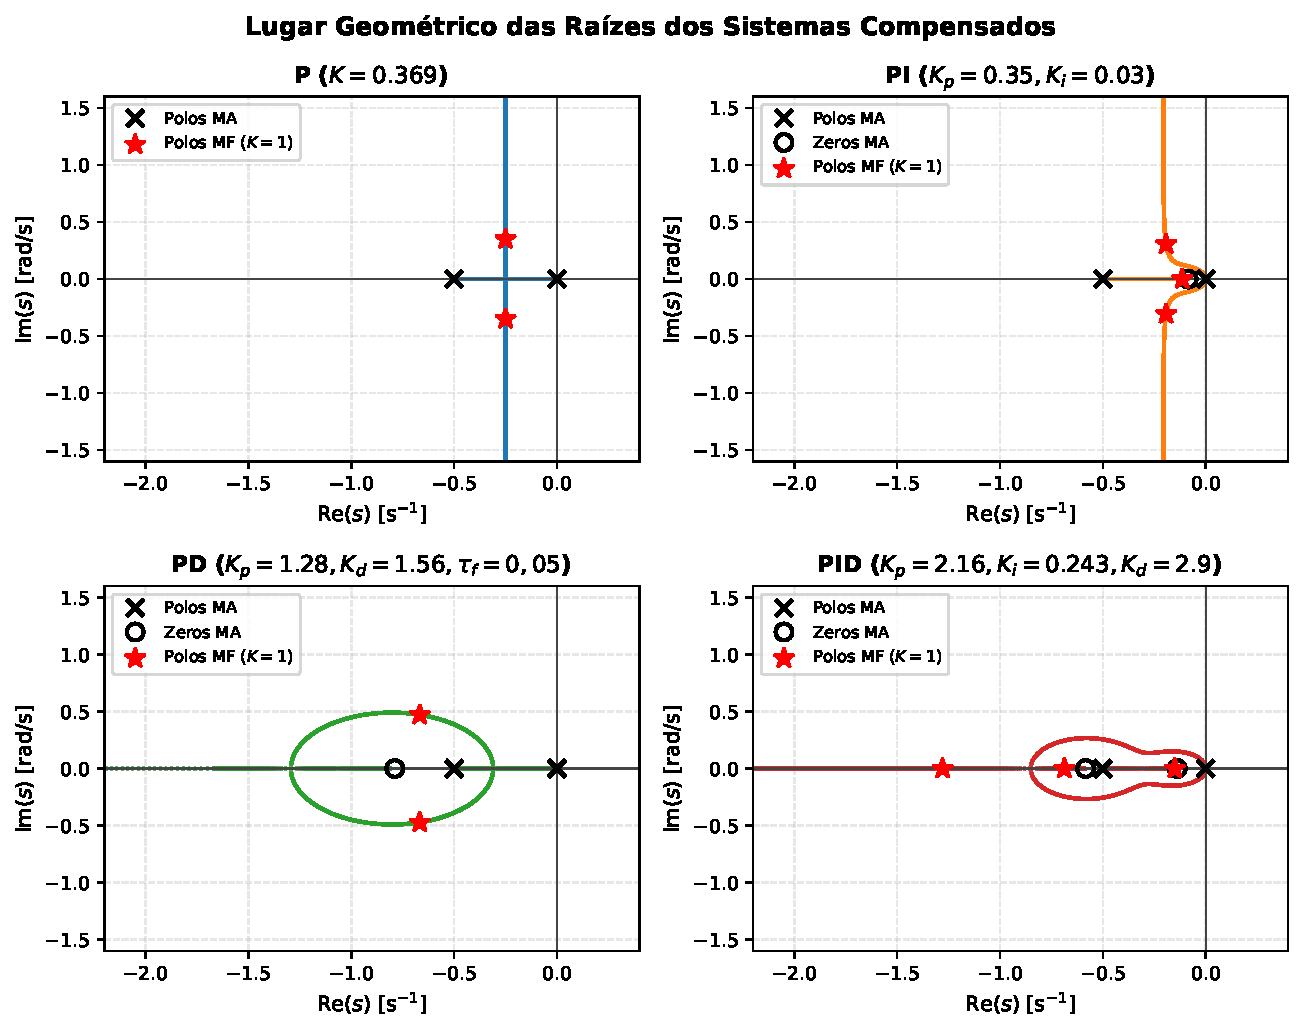
\includegraphics[width=0.76\textwidth]{figuras/fig4_lgr_compensadores.pdf}%
    }{%
        \fbox{\parbox{0.80\textwidth}{\centering\vspace{1.0cm}\textit{[Aguardando \texttt{figuras/fig4\_lgr\_compensadores.pdf}]}\vspace{1.0cm}}}%
    }
    \fontefig{Fonte: Elaborada pelos autores com base nos resultados de simulação (2026).}
\end{figure}

\begin{figure}[H]
    \centering
    \caption{Diagramas de Bode das funções de transferência de malha aberta compensada $L(j\omega)$ para P, PI, PD e PID com indicação das margens de ganho ($\mathrm{GM}$) e de fase ($\mathrm{PM}$)}
    \label{fig:bode_comp}
    \IfFileExists{figuras/fig5_bode_compensadores.pdf}{%
        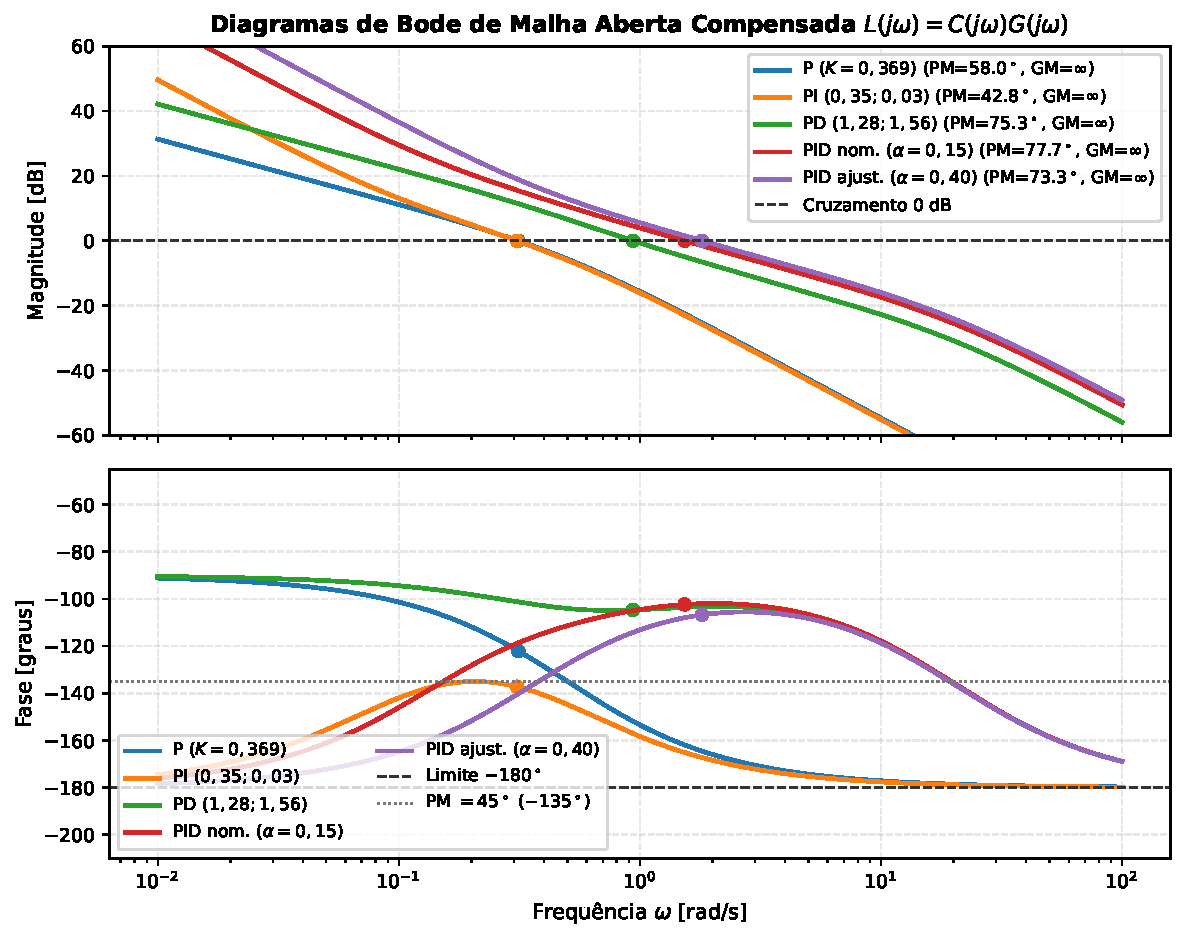
\includegraphics[width=0.76\textwidth]{figuras/fig5_bode_compensadores.pdf}%
    }{%
        \fbox{\parbox{0.80\textwidth}{\centering\vspace{1.0cm}\textit{[Aguardando \texttt{figuras/fig5\_bode\_compensadores.pdf}]}\vspace{1.0cm}}}%
    }
    \fontefig{Fonte: Elaborada pelos autores com base nos resultados de simulação (2026).}
\end{figure}

\subsection{Demonstração Matemática e Evidências Computacionais das Limitações}\label{sec:limitacoes_comp}

\subsubsection{Limitação Estrutural do Controlador PI (Invariância de Vieta e Instabilidade)}
Na equação característica mônica da malha fechada com PI,
\begin{equation}
    s^3 + 0{,}5\,s^2 + \frac{K_p}{2}\,s + \frac{K_i}{2} = 0,
\end{equation}
as relações de Vieta impõem que a soma das três raízes $p_1, p_2, p_3$ seja independente de $K_p$ e $K_i$:
\begin{equation}
    p_1 + p_2 + p_3 = -0{,}5\text{ s}^{-1} \implies \bar{\sigma} = \frac{\operatorname{Re}(p_1) + \operatorname{Re}(p_2) + \operatorname{Re}(p_3)}{3} = -\frac{1}{6} \approx -0{,}167\text{ s}^{-1}.
\end{equation}
Para qualquer par estabilizante ($K_i < K_p/2$, de modo que $\operatorname{Re}(p_k) < 0\;\forall k$), pelo menos um polo deve satisfazer $\operatorname{Re}(p_k) \ge -1/6\text{ s}^{-1}$. Consequentemente, a constante de tempo dominante é no mínimo $\tau_{\text{dom}} \ge 6\text{ s}$, acarretando tempo de acomodação elevado (no projeto estável $K_p=0{,}35,\,K_i=0{,}03$, obtém-se $p_{1,2}=-0{,}193\pm j0{,}306$ e $p_3=-0{,}115$, resultando em $t_s=19{,}578\text{ s} > 12\text{ s}$, $M_p=34{,}67\% > 10\%$ e $\mathrm{PM}=42{,}78^\circ < 45^\circ$). Quando se viola o critério de Routh-Hurwitz tomando $K_i = 0{,}30 \ge K_p/2 = 0{,}25$ ($K_p=0{,}50$), dois polos migram para o semiplano direito em $+0{,}023 \pm j\,0{,}524\text{ s}^{-1}$ ($\mathrm{PM} = -5{,}21^\circ$), tornando o sistema instável: na simulação linear ocorre divergência oscilatória crescente e, sob saturação com restrição $q(t)\ge 0$, instala-se um ciclo limite auto-sustentado (Figura~\ref{fig:pid_windup}, painéis inferiores). Para configurações instáveis, métricas de regime transitório ($t_r, t_s, M_p$) e erro estacionário ($e_{ss}$) não se aplicam.

\subsubsection{Limitação do Controlador PD (Rejeição à Perturbação vs. Saturação)}
Como $C_{\text{PD}}(s)$ não possui integrador, e o integrador da planta situa-se a jusante do ponto de entrada da perturbação, a malha não rejeita completamente a perturbação em degrau $\Delta\lambda(t) = 100\,\mathbb{1}(t - 20)$:
\begin{equation}
    e_{ss,\text{dist}} = \lim_{s\to 0} s\left(\frac{2s+1}{2s^2 + (1+K_d)s + K_p}\right)\frac{100}{s} = \frac{100}{K_p}.
\end{equation}
Como $K_p = 2\omega_n^2$, cumprir $e_{ss,\text{dist}} \le 10\text{ eventos}$ exige $K_p \ge 10$ ($\omega_n \ge \sqrt{5} \approx 2{,}24\text{ rad/s}$). Todavia, em $t = 0^+$, um erro inicial de $x_r = 300\text{ eventos}$ provoca esforço proporcional $u_P(0^+) = 300 K_p \ge 3000\text{ eventos/s}$ ($\mu_c(0^+) \ge 4000\text{ eventos/s}$), excedendo em quase três vezes o limite físico de $1400\text{ eventos/s}$, sem contar o pico adicional da ação derivativa quando aplicada ao erro. Com a sintonia adotada ($K_p = 1{,}280$, $K_d = 1{,}560$), a partida é rápida ($t_s = 6{,}018\text{ s}$, $M_p = 4{,}70\%$), mas o erro após a perturbação estabiliza em $100/1{,}28 \approx 78{,}13\text{ eventos}$; mesmo a sintonia mais agressiva $K_p = 2{,}000$, $K_d = 2{,}400$ ($\omega_n = 1{,}0\text{ rad/s}$, $\zeta = 0{,}85$) ainda deixa $50{,}00\text{ eventos}$, cinco vezes o teto admitido.

\subsubsection[Limitações Não Lineares no Controlador PID]{Limitações Não Lineares no Controlador PID (Saturação, \textit{Windup} e Sensibilidade Derivativa)}
Embora o PID rompa a invariância da soma dos polos ($p_1+p_2+p_3 = -(1+K_d)/2$) e anule $e_{ss,\text{dist}}$, sua operação com atuador limitado expõe fenômenos não lineares discutidos na literatura de controle industrial (ÅSTRÖM; HÄGGLUND, 2006; FRANKLIN; POWELL; EMAMI-NAEINI, 2013) e ilustrados nos painéis superiores da Figura~\ref{fig:pid_windup}. O primeiro é a própria saturação. Como a capacidade admite incremento máximo de $+400\text{ eventos/s}$, a taxa inicial de drenagem da fila fica limitada, e o tempo de subida do PID nominal passa de $1{,}022\text{ s}$ no modelo linear para $2{,}236\text{ s}$ com saturação sem \textit{anti-windup} e para $2{,}802\text{ s}$ com \textit{back-calculation} e derivada na medição.

A saturação provoca, por sua vez, o \textit{windup} integral. Sem proteção, o integrador continua acumulando erro positivo durante os $0{,}502\text{ s}$ em que $\mu_c > 1400\text{ eventos/s}$, e o sobressinal sobe de $8{,}13\%$ para $15{,}79\%$, com tempo de acomodação de $21{,}680\text{ s}$. O \textit{clamping} reduz o sobressinal para $12{,}19\%$, valor que ainda viola a especificação. O \textit{back-calculation} com $T_t = 0{,}5\text{ s}$ leva o sobressinal a $6{,}50\%$ no PID nominal e a $6{,}98\%$, com $t_s = 10{,}744\text{ s}$, no PID ajustado ($\alpha = 0{,}40\text{ s}^{-1}$).

O terceiro fenômeno vem da sensibilidade da ação derivativa a variações bruscas do erro. Quando a derivada incide sobre $e(t) = x_r - x(t)$, o degrau de referência gera em $t = 0^+$ um pico de $\mu_c = 19048\text{ eventos/s}$ no PID nominal e de $10744\text{ eventos/s}$ no PD, mesmo com o filtro $\tau_f = 0{,}05\text{ s}$ (\textit{derivative kick}). Com a derivada aplicada somente à medição, $-K_d s\,X(s)/(\tau_f s+1)$, o incremento solicitado reduz-se de $18048$ para $648\text{ eventos/s}$ no PID nominal e de $9744$ para $384\text{ eventos/s}$ no PD, que deixa de saturar. O filtro, por sua vez, continua atenuando o ruído de medição em alta frequência.

\begin{figure}[H]
    \centering
    \caption{Evidências computacionais das limitações dinâmicas e não lineares: (acima) efeito da saturação, \textit{windup}, \textit{anti-windup} (\textit{clamping} e \textit{back-calculation}) e \textit{derivative kick} em escala logarítmica para o PID; (abaixo) divergência linear e ciclo limite sob saturação no PI instável ($K_p=0{,}50,\,K_i=0{,}30$)}
    \label{fig:pid_windup}
    \IfFileExists{figuras/fig8_pid_windup_derivativa.pdf}{%
        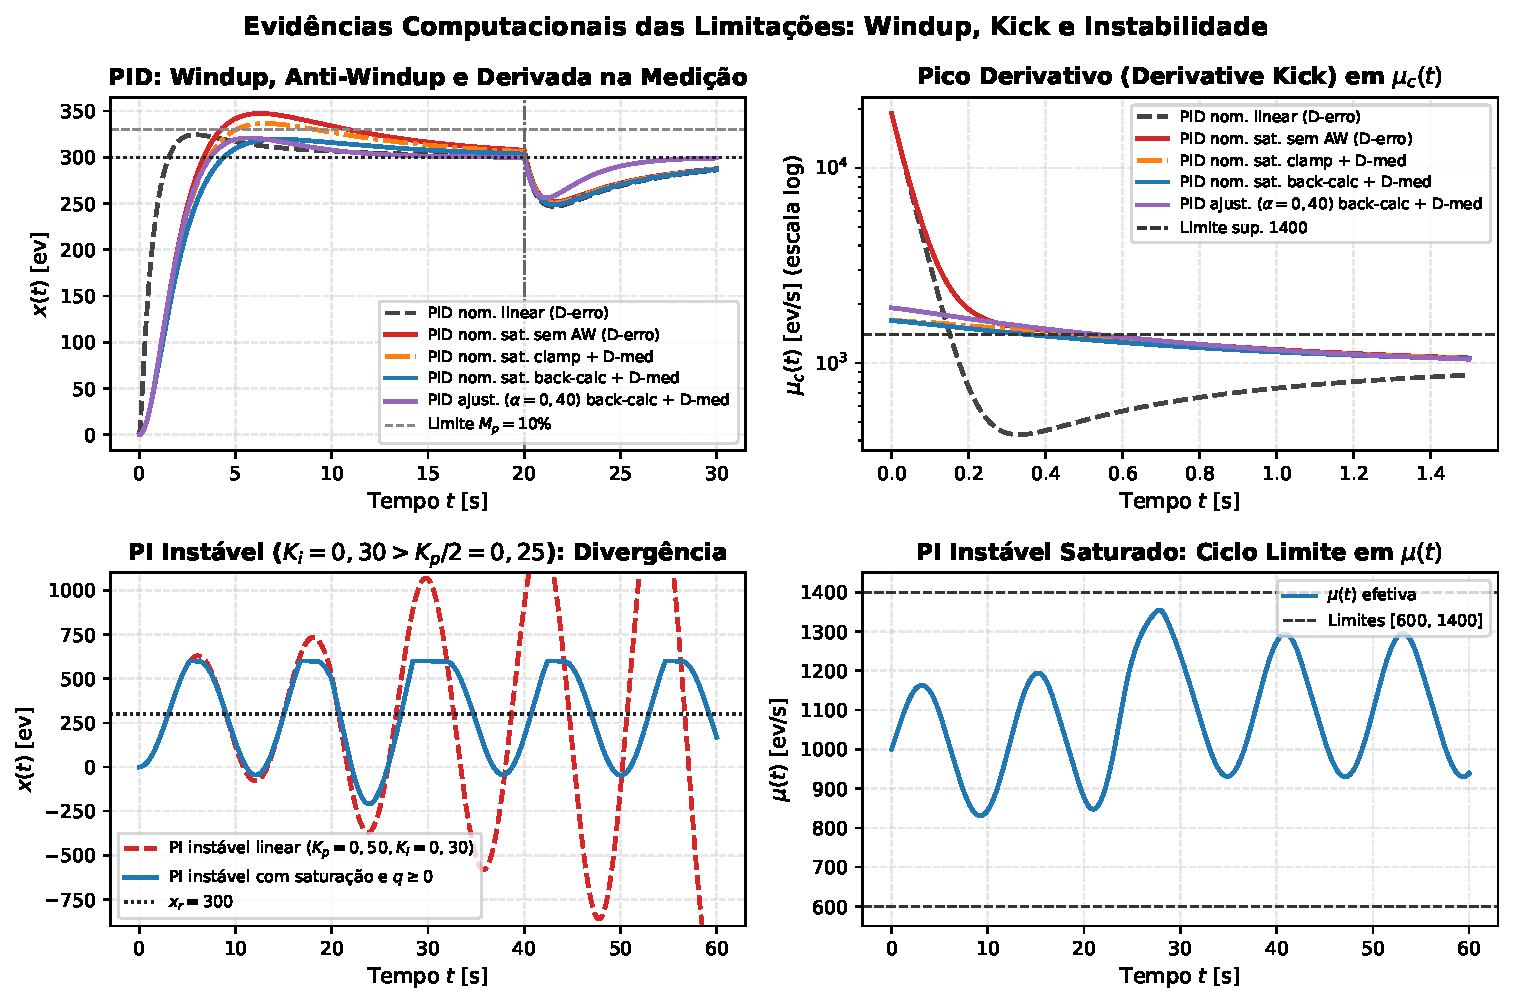
\includegraphics[width=0.78\textwidth]{figuras/fig8_pid_windup_derivativa.pdf}%
    }{%
        \fbox{\parbox{0.80\textwidth}{\centering\vspace{1.0cm}\textit{[Aguardando \texttt{figuras/fig8\_pid\_windup\_derivativa.pdf}]}\vspace{1.0cm}}}%
    }
    \fontefig{Fonte: Elaborada pelos autores com base nos resultados de simulação (2026).}
\end{figure}
